%  LaTeX support: latex@mdpi.com 
\documentclass[metlit,article,accept,pdftex,moreauthors]{Definitions/mdpi} 
\usepackage{caption}
\usepackage{subcaption}
\usepackage[indonesian]{babel}

\firstpage{1} 
\makeatletter 
\setcounter{page}{\@firstpage} 
\makeatother
\pubvolume{1}
\issuenum{1}
\articlenumber{0}
\pubyear{2026}
\copyrightyear{2026}
\datereceived{20 Maret 2026} 
\dateaccepted{22 Maret 2026} 
\datepublished{ } 
\hreflink{https://doi.org/}

%=================================================================
\Title{Pengaruh Screen Time terhadap Kualitas Tidur Mahasiswa: Studi Kuantitatif Menggunakan Uji-Z untuk Selisih Dua Rata-rata}

\TitleCitation{Pengaruh Screen Time terhadap Kualitas Tidur Mahasiswa}

\newcommand{\orcidauthorA}{0000-0000-0000-000X}

\Author{Syahril Arfian Almazril}

\AuthorNames{Syahril Arfian Almazril}

\AuthorCitation{Almazril, S.A.}

\address{%
$^{1}$ \quad Teknologi Informasi, Telkom University, Bandung, Indonesia\\
}

\corres{Correspondence: arfazrll@student.telkomuniversity.ac.id}


\abstract{Penelitian ini bertujuan untuk menganalisis pengaruh \textit{screen time} terhadap kualitas tidur mahasiswa. Data dikumpulkan dari 150 responden mahasiswa yang melaporkan durasi penggunaan layar harian dan skor kualitas tidur (skala 1--10). Responden dikelompokkan menjadi dua kategori: \textit{screen time} tinggi ({$>$}6 jam/hari, n=52) dan \textit{screen time} non-tinggi ($\leq$6 jam/hari, n=98). Pengujian hipotesis dilakukan menggunakan uji-Z untuk selisih dua rata-rata. Hasil analisis menunjukkan bahwa kelompok \textit{screen time} tinggi memiliki rata-rata kualitas tidur sebesar 4,68, sedangkan kelompok non-tinggi sebesar 6,49. Nilai statistik uji yang diperoleh adalah $z = -7{,}96$ dengan $p$-value $\approx 0{,}0000$, yang jauh lebih kecil dari tingkat signifikansi $\alpha = 0{,}05$. Dengan demikian, hipotesis nol ditolak dan disimpulkan bahwa terdapat perbedaan signifikan dalam kualitas tidur antara kedua kelompok. Koefisien korelasi Pearson antara \textit{screen time} dan kualitas tidur adalah $r = -0{,}75$, mengindikasikan hubungan negatif yang kuat.}

\keyword{\textit{screen time}; kualitas tidur; uji-Z; mahasiswa; pengujian hipotesis}

%%%%%%%%%%%%%%%%%%%%%%%%%%%%%%%%%%%%%%%%%%
\begin{document}

%%%%%%%%%%%%%%%%%%%%%%%%%%%%%%%%%%%%%%%%%%
\section{Pendahuluan}

Di era digital saat ini, perangkat elektronik seperti \textit{smartphone}, laptop, dan tablet telah menjadi bagian yang tidak terpisahkan dari kehidupan mahasiswa. Menurut laporan World Health Organization \cite{WHO2024screentime}, penggunaan layar digital di kalangan anak muda meningkat secara signifikan dalam dekade terakhir. Fenomena ini menimbulkan kekhawatiran terhadap dampak kesehatan, khususnya kualitas tidur yang merupakan faktor penting dalam performa akademik dan kesejahteraan fisik maupun mental.

Beberapa penelitian sebelumnya telah menunjukkan bahwa paparan cahaya biru dari layar digital dapat menekan produksi hormon melatonin, yang berperan dalam mengatur siklus tidur-bangun atau ritme sirkadian \cite{chang2015evening}. Hale dan Guan \cite{hale2015screen} melalui tinjauan sistematis menemukan hubungan konsisten antara penggunaan layar dan gangguan tidur pada remaja. Namun, penelitian spesifik mengenai dampak \textit{screen time} terhadap kualitas tidur mahasiswa di Indonesia masih terbatas.

Berdasarkan latar belakang tersebut, penelitian ini mengajukan pertanyaan penelitian sebagai berikut: \textit{Apakah terdapat perbedaan kualitas tidur yang signifikan antara mahasiswa dengan screen time tinggi ({$>$}6 jam/hari) dan mahasiswa dengan screen time non-tinggi ($\leq$6 jam/hari)?} Pertanyaan ini bersifat netral tanpa mengasumsikan arah tertentu, sesuai dengan prinsip penyusunan \textit{research question} yang baik.

Hipotesis yang diajukan dalam penelitian ini adalah sebagai berikut. Hipotesis nol ($H_0$) menyatakan bahwa tidak ada perbedaan rata-rata kualitas tidur antara kedua kelompok, atau secara formal $\mu_A - \mu_B = 0$. Hipotesis alternatif ($H_1$) menyatakan bahwa terdapat perbedaan rata-rata kualitas tidur antara kedua kelompok, yaitu $\mu_A - \mu_B \neq 0$. Pengujian dilakukan menggunakan uji-Z dua arah (\textit{two-tailed}) dengan tingkat signifikansi $\alpha = 0{,}05$.

Struktur penulisan artikel ini adalah sebagai berikut. Bagian 2 membahas penelitian terkait mengenai hubungan \textit{screen time} dan kualitas tidur. Bagian 3 menjelaskan metodologi penelitian termasuk pengumpulan data dan rumus statistik yang digunakan. Bagian 4 menyajikan hasil percobaan dan analisis statistik. Bagian 5 menutup artikel dengan kesimpulan.

\section{Penelitian Terkait}

Hubungan antara penggunaan perangkat digital dan kualitas tidur telah menjadi topik penelitian yang aktif dalam beberapa tahun terakhir. Carter dkk. \cite{carter2016association} melakukan meta-analisis terhadap 20 studi dan menemukan bahwa penggunaan perangkat layar portabel secara konsisten berhubungan dengan berkurangnya kuantitas dan kualitas tidur. Hasil meta-analisis tersebut menunjukkan bahwa pengguna aktif perangkat layar memiliki risiko dua kali lipat mengalami kualitas tidur yang buruk dibandingkan non-pengguna.

Exelmans dan Van den Bulck \cite{exelmans2016bedtime} meneliti penggunaan \textit{smartphone} sebelum tidur pada populasi dewasa di Belgia. Studi tersebut menemukan bahwa penggunaan \textit{smartphone} di tempat tidur berkorelasi positif dengan latensi tidur yang lebih lama, kualitas tidur yang lebih buruk, dan rasa kantuk di siang hari. Temuan ini sejalan dengan penelitian Fossum dkk. \cite{fossum2014association} yang menunjukkan bahwa penggunaan media elektronik di tempat tidur berhubungan dengan gejala insomnia.

Christensen dkk. \cite{christensen2016direct} menggunakan pengukuran langsung terhadap \textit{screen time smartphone} dan menemukan bahwa rata-rata durasi penggunaan harian mencapai 3,7 jam pada populasi dewasa muda. Studi tersebut juga mengungkapkan korelasi negatif antara durasi penggunaan dan kualitas tidur yang dilaporkan sendiri. Demirci dkk. \cite{demirci2015relationship} secara khusus meneliti mahasiswa dan menemukan hubungan signifikan antara keparahan penggunaan \textit{smartphone}, kualitas tidur, depresi, dan kecemasan.

Dari sisi mekanisme biologis, Chang dkk. \cite{chang2015evening} membuktikan bahwa paparan cahaya dari \textit{e-reader} pada malam hari secara signifikan menekan produksi melatonin, menggeser ritme sirkadian, dan mengurangi kewaspadaan di pagi hari. Gradisar dkk. \cite{gradisar2013sleep} melalui survei nasional di Amerika Serikat menemukan bahwa 95\% responden menggunakan perangkat elektronik dalam satu jam sebelum tidur, dan hal ini berhubungan dengan berkurangnya durasi dan kualitas tidur.

Berdasarkan tinjauan literatur di atas, terlihat bahwa mayoritas studi dilakukan di negara-negara Barat. Penelitian ini bertujuan mengisi celah tersebut dengan menganalisis dampak \textit{screen time} terhadap kualitas tidur mahasiswa menggunakan pendekatan pengujian hipotesis statistik, khususnya uji-Z untuk selisih dua rata-rata.

\section{Metodologi}

\subsection{Alur Penelitian}

Metodologi penelitian ini mengikuti alur sistematis yang dimulai dari identifikasi masalah hingga pengambilan kesimpulan. Gambar~\ref{fig:flowchart} mengilustrasikan diagram alir penelitian yang digunakan. Setiap tahap dilaksanakan secara berurutan untuk memastikan validitas hasil penelitian.

\begin{figure}[H]
    \centering
    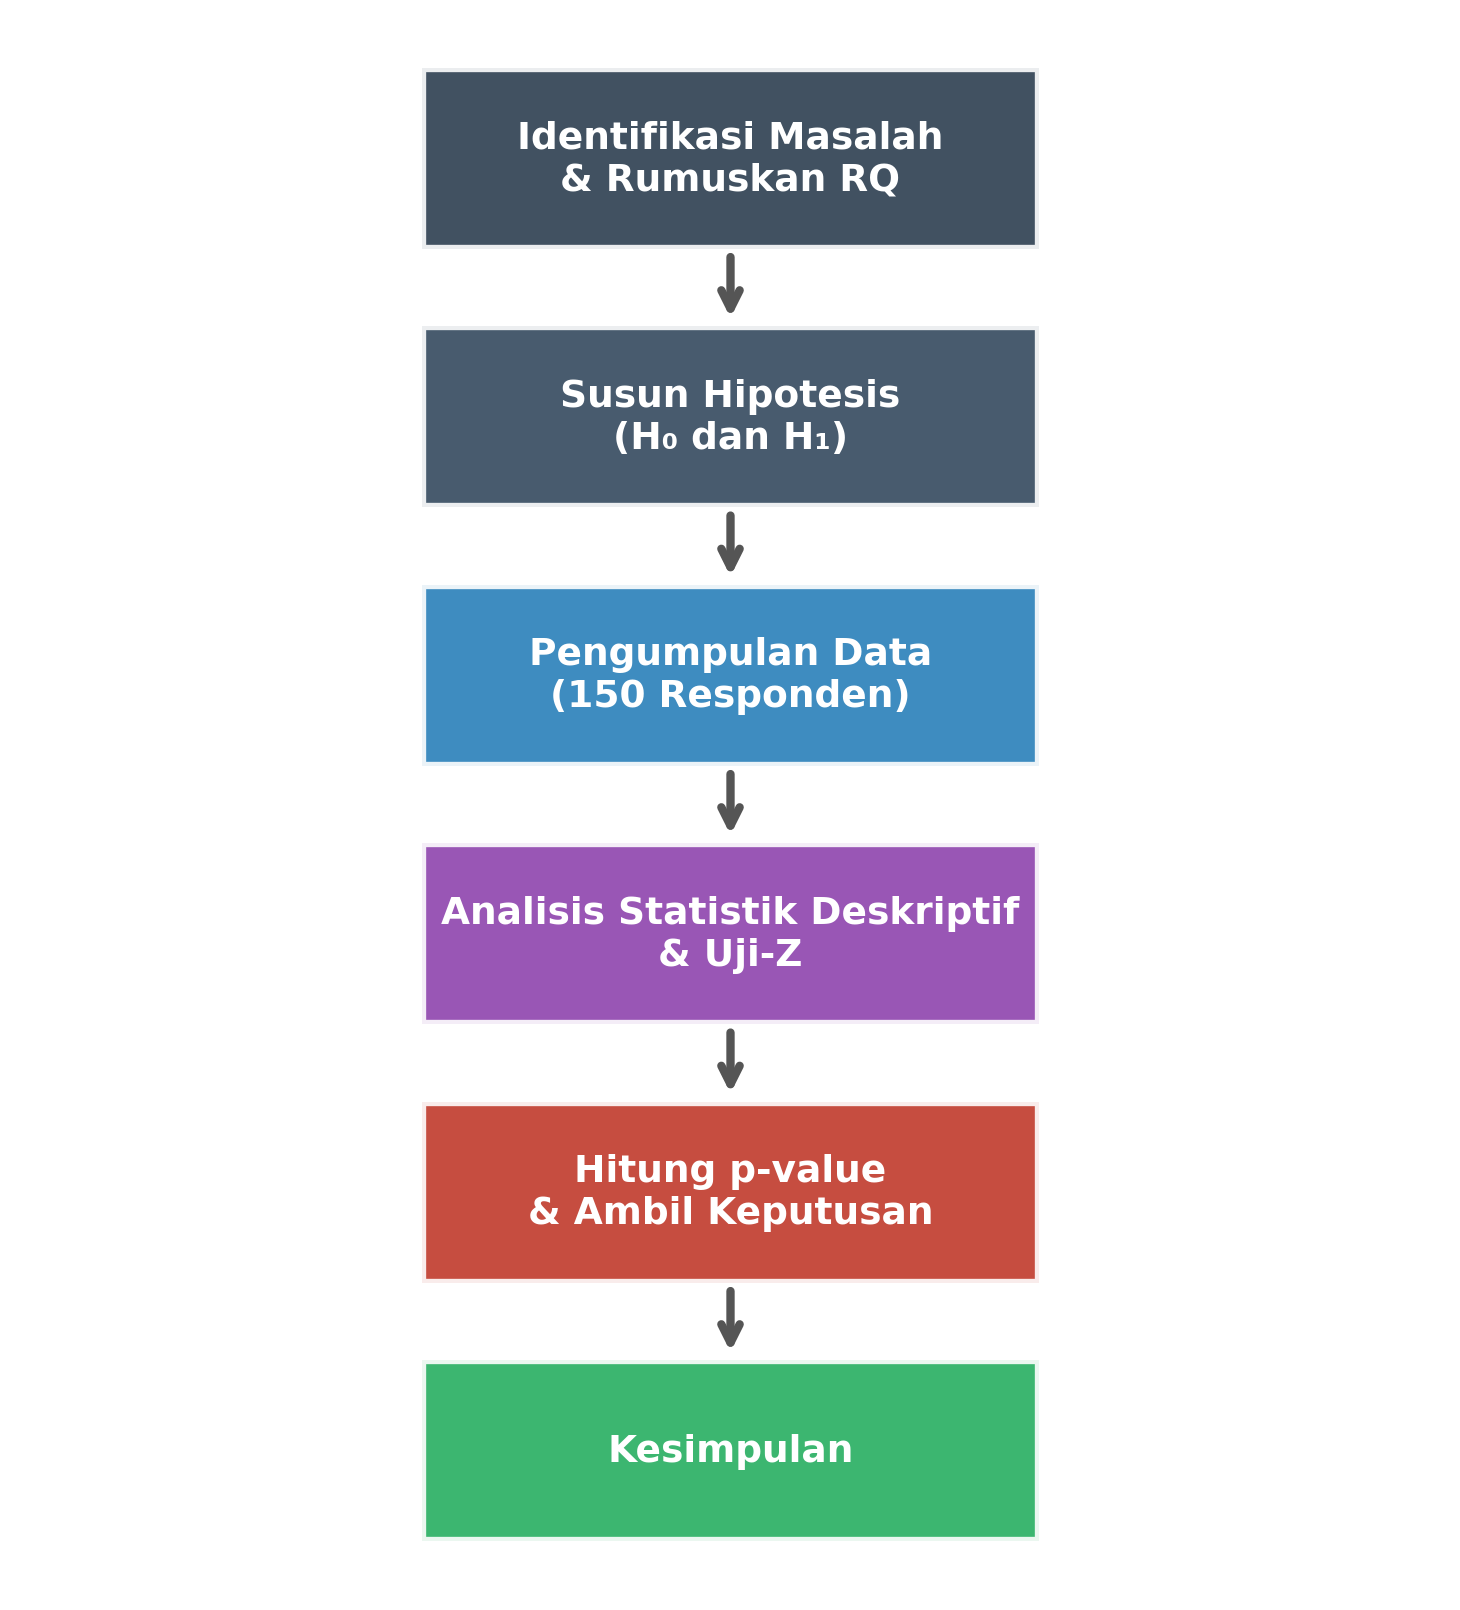
\includegraphics[width=0.6\linewidth]{image_rev/diagram_flowchart.png}
    \caption{Diagram alir metodologi penelitian.}
    \label{fig:flowchart}
\end{figure}

\subsection{Pengumpulan Data}

Data dikumpulkan dari 150 mahasiswa melalui kuesioner yang mencakup informasi demografis, durasi \textit{screen time} harian (dalam jam), dan skor kualitas tidur yang dilaporkan sendiri dalam skala 1--10. Responden terdiri dari 68 laki-laki (45,3\%) dan 82 perempuan (54,7\%). Berdasarkan durasi \textit{screen time}, responden dikelompokkan menjadi tiga kategori: tinggi ({$>$}6 jam, $n=52$), sedang (3--6 jam, $n=79$), dan rendah ($\leq$3 jam, $n=19$).

\subsection{Rumus Statistik}

Untuk menguji hipotesis penelitian, digunakan uji-Z untuk selisih dua rata-rata independen. Metode ini dipilih karena ukuran sampel kedua kelompok cukup besar ($n > 30$), sehingga distribusi sampling mendekati distribusi normal sesuai Teorema Limit Pusat \cite{moore2016basic}. Langkah-langkah perhitungan adalah sebagai berikut.

Pertama, untuk masing-masing kelompok $k \in \{A, B\}$, dihitung rata-rata sampel dan simpang baku:
\begin{equation}
\label{eq:mean}
\bar{x}_k = \frac{1}{N_k}\sum_{i=1}^{N_k} x_{k,i}, \quad \sigma_k = \sqrt{\frac{1}{N_k}\sum_{i=1}^{N_k}(x_{k,i} - \bar{x}_k)^2}
\end{equation}
di mana $N_k$ adalah jumlah sampel kelompok $k$ dan $x_{k,i}$ adalah nilai kualitas tidur responden ke-$i$ pada kelompok tersebut.

Selanjutnya, \textit{Standard Error of the Mean} (SEM) dan \textit{Standard Error of Difference} dihitung sebagai:
\begin{equation}
\label{eq:sem}
\text{SEM}_k = \frac{\sigma_k}{\sqrt{N_k}}, \quad SE_{A-B} = \sqrt{\text{SEM}_A^2 + \text{SEM}_B^2}
\end{equation}

Nilai statistik uji $z$ kemudian dihitung menggunakan:
\begin{equation}
\label{eq:ztest}
z = \frac{\Delta\bar{x} - 0}{SE_{A-B}} = \frac{(\bar{x}_A - \bar{x}_B)}{SE_{A-B}}
\end{equation}

Terakhir, $p$-value diperoleh dari tabel distribusi normal standar (Tabel Z). Karena pengujian bersifat dua arah (\textit{two-tailed}), maka $p\text{-value} = 2 \times P(Z \leq z)$ untuk $z < 0$. Keputusan diambil dengan membandingkan $p$-value terhadap tingkat signifikansi $\alpha = 0{,}05$: jika $p\text{-value} < \alpha$, maka $H_0$ ditolak.

\section{Hasil Percobaan}

\subsection{Statistik Deskriptif}

Tabel~\ref{tab:deskriptif} menyajikan ringkasan statistik deskriptif untuk setiap kategori \textit{screen time}. Secara umum, rata-rata \textit{screen time} seluruh responden adalah 5,34 jam/hari dengan rata-rata kualitas tidur 5,86. Terlihat pola yang jelas: semakin tinggi \textit{screen time}, semakin rendah skor kualitas tidur.

\begin{table}[H]
\centering
\caption{Statistik deskriptif berdasarkan kategori \textit{screen time}.}
\label{tab:deskriptif}
\begin{tabular}{@{}lccc@{}}
\toprule
\textbf{Kategori} & \textbf{n} & \textbf{Rata-rata ST (jam)} & \textbf{Rata-rata QT (skor)} \\
\midrule
Rendah ($\leq$3 jam) & 19 & 2,31 & 7,39 \\
Sedang (3--6 jam) & 79 & 4,77 & 6,28 \\
Tinggi ({$>$}6 jam) & 52 & 7,31 & 4,68 \\
\midrule
\textbf{Total} & \textbf{150} & \textbf{5,34} & \textbf{5,86} \\
\bottomrule
\end{tabular}
\end{table}

Kelompok \textit{screen time} rendah memiliki skor kualitas tidur tertinggi (7,39), sedangkan kelompok tinggi memiliki skor terendah (4,68). Selisih kualitas tidur antara kelompok rendah dan tinggi mencapai 2,71 poin, menunjukkan perbedaan yang substansial secara deskriptif.

Gambar~\ref{fig:scatter} menampilkan diagram sebar hubungan antara \textit{screen time} dan kualitas tidur untuk seluruh 150 responden. Pola yang terlihat menunjukkan kecenderungan menurun: semakin tinggi durasi \textit{screen time}, semakin rendah kualitas tidur yang dilaporkan. Koefisien korelasi Pearson yang diperoleh adalah $r = -0{,}75$, mengindikasikan hubungan negatif yang kuat antara kedua variabel.

\begin{figure}[H]
    \centering
    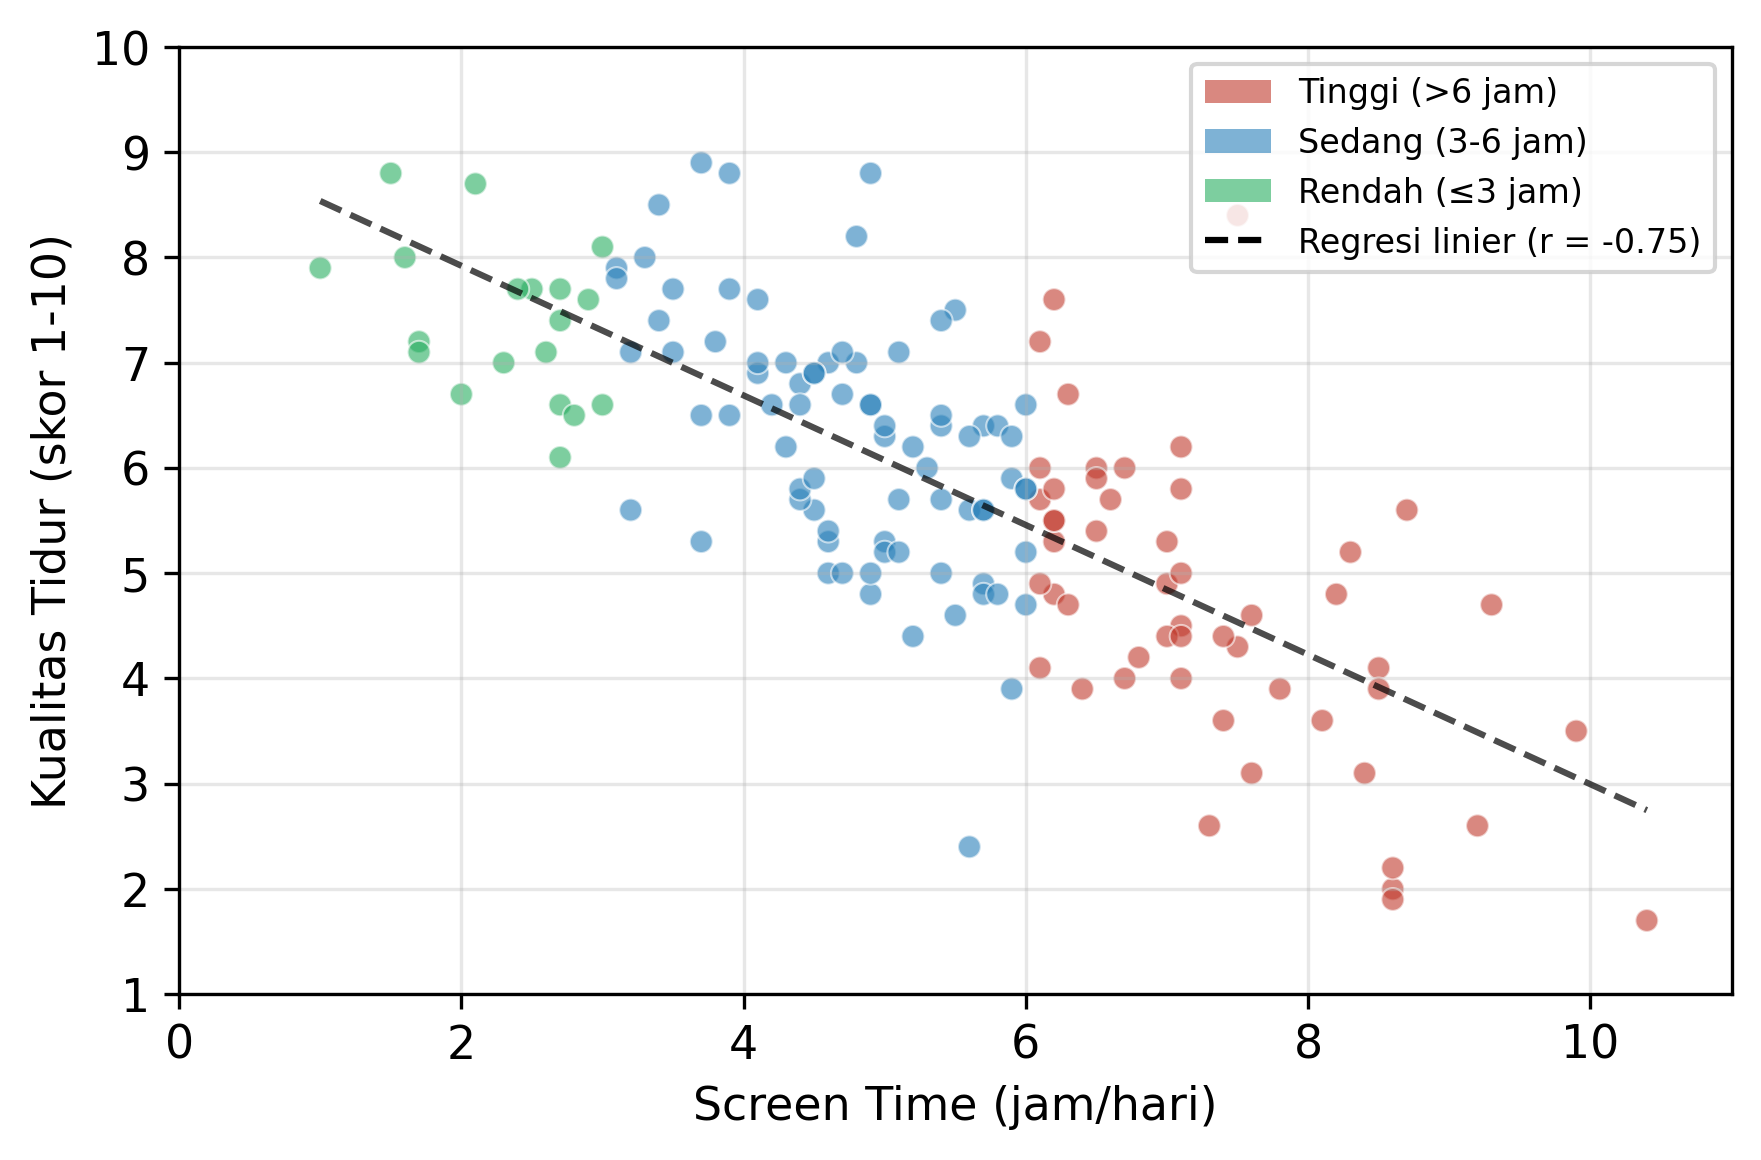
\includegraphics[width=0.75\linewidth]{image_rev/scatter_screentime.png}
    \caption{Diagram sebar \textit{screen time} vs. kualitas tidur ($r = -0{,}75$).}
    \label{fig:scatter}
\end{figure}

\subsection{Pengujian Hipotesis}

Pengujian hipotesis dilakukan untuk membandingkan rata-rata kualitas tidur antara kelompok \textit{screen time} tinggi (Grup A, $n_A = 52$) dan kelompok non-tinggi (Grup B, $n_B = 98$). Tabel~\ref{tab:uji} menyajikan hasil perhitungan statistik kedua kelompok.

\begin{table}[H]
\centering
\caption{Hasil perhitungan statistik untuk uji-Z.}
\label{tab:uji}
\begin{tabular}{@{}lcc@{}}
\toprule
\textbf{Statistik} & \textbf{Grup A (ST Tinggi)} & \textbf{Grup B (ST Non-Tinggi)} \\
\midrule
Jumlah sampel ($n$) & 52 & 98 \\
Rata-rata ($\bar{x}$) & 4,6769 & 6,4939 \\
Simpang baku ($\sigma$) & 1,3990 & 1,1899 \\
SEM ($\sigma/\sqrt{n}$) & 0,1940 & 0,1202 \\
\bottomrule
\end{tabular}
\end{table}

Berdasarkan data pada Tabel~\ref{tab:uji}, perhitungan dilakukan menggunakan Persamaan~\eqref{eq:sem} dan~\eqref{eq:ztest} sebagai berikut:

\begin{itemize}
    \item \textbf{Standard Error of Difference:}
    $SE_{A-B} = \sqrt{0{,}1940^2 + 0{,}1202^2} = \sqrt{0{,}037638 + 0{,}014448} = \mathbf{0{,}2282}$
    \item \textbf{Selisih rata-rata sampel:}
    $\Delta\bar{x} = \bar{x}_A - \bar{x}_B = 4{,}6769 - 6{,}4939 = \mathbf{-1{,}8170}$
    \item \textbf{Statistik uji:}
    $z = \frac{-1{,}8170 - 0}{0{,}2282} = \mathbf{-7{,}9613}$
    \item \textbf{p-value:} Karena $|z| = 7{,}96$ jauh melampaui batas Tabel Z (pada $z = -3{,}6$, $P = 0{,}0002$), maka $p\text{-value} = 2 \times P(Z \leq -7{,}96) \approx 2 \times 0{,}0000 = \mathbf{0{,}0000}$
\end{itemize}

\subsection{Keputusan dan Interpretasi}

Karena $p\text{-value} \approx 0{,}0000 < \alpha = 0{,}05$, maka \textbf{hipotesis nol ($H_0$) ditolak}. Dengan demikian, hipotesis alternatif ($H_1$) diterima: terdapat perbedaan yang signifikan secara statistik dalam rata-rata kualitas tidur antara mahasiswa dengan \textit{screen time} tinggi dan non-tinggi.

Gambar~\ref{fig:boxplot} memvisualisasikan distribusi kualitas tidur untuk ketiga kategori \textit{screen time}. Pola penurunan yang konsisten terlihat jelas dari kelompok rendah menuju tinggi, mendukung hasil pengujian hipotesis yang telah dilakukan.

\begin{figure}[H]
    \centering
    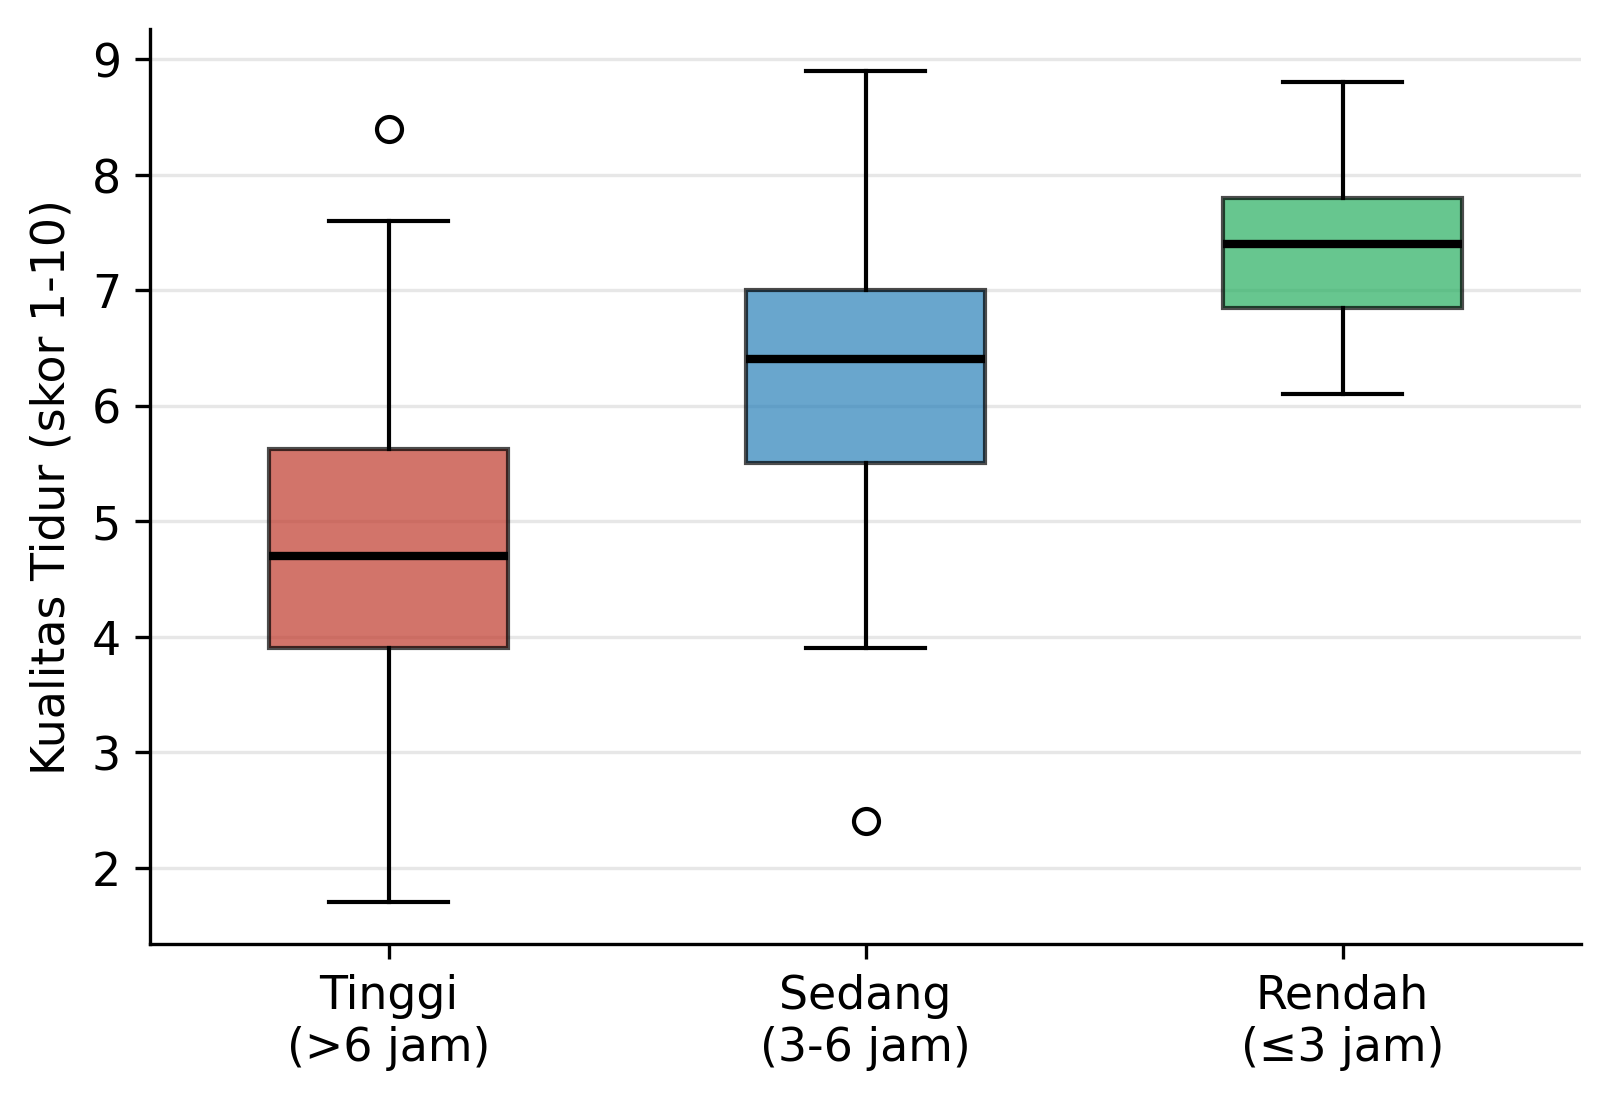
\includegraphics[width=0.75\linewidth]{image_rev/gambar_hasil.png}
    \caption{Distribusi kualitas tidur berdasarkan kategori \textit{screen time}.}
    \label{fig:boxplot}
\end{figure}

Secara praktis, perbedaan 1,82 poin (pada skala 1--10) antara kelompok \textit{screen time} tinggi dan non-tinggi merupakan selisih yang cukup besar. Nilai korelasi $r = -0{,}75$ juga menunjukkan bahwa \textit{screen time} dapat menjelaskan sekitar 56\% variasi dalam kualitas tidur ($r^2 = 0{,}56$). Temuan ini konsisten dengan literatur sebelumnya yang menunjukkan dampak negatif penggunaan layar berlebihan terhadap kualitas tidur.

\section{Simpulan}

Penelitian ini menganalisis pengaruh \textit{screen time} terhadap kualitas tidur mahasiswa menggunakan data dari 150 responden dan uji-Z untuk selisih dua rata-rata. Hasil pengujian menunjukkan nilai $z = -7{,}96$ dengan $p$-value $\approx 0{,}0000$, sehingga hipotesis nol ditolak pada tingkat signifikansi $\alpha = 0{,}05$. Terdapat perbedaan yang signifikan secara statistik antara rata-rata kualitas tidur mahasiswa dengan \textit{screen time} tinggi ($\bar{x} = 4{,}68$) dan non-tinggi ($\bar{x} = 6{,}49$).

Koefisien korelasi Pearson sebesar $r = -0{,}75$ mengkonfirmasi hubungan negatif yang kuat antara durasi penggunaan layar dan kualitas tidur. Temuan ini sejalan dengan penelitian-penelitian sebelumnya \cite{hale2015screen,carter2016association,chang2015evening} dan memberikan bukti empiris untuk konteks mahasiswa di Indonesia. Implikasi praktis dari penelitian ini adalah pentingnya manajemen waktu layar bagi mahasiswa untuk menjaga kualitas tidur yang optimal.

%%%%%%%%%%%%%%%%%%%%%%%%%%%%%%%%%%%%%%%%%%
\vspace{6pt} 

\acknowledgments{Penulis mengucapkan terima kasih kepada dosen pengampu mata kuliah Metode Penelitian atas bimbingan dalam penyusunan artikel ini.}

\conflictsofinterest{Penulis menyatakan tidak ada konflik kepentingan.} 

\useofartificialintelligence{Pengembangan paragraf pada bagian Penelitian Terkait dan Pendahuluan dibantu oleh AI. Seluruh ide inti, analisis data, perhitungan statistik, dan interpretasi hasil merupakan karya penulis.}

%%%%%%%%%%%%%%%%%%%%%%%%%%%%%%%%%%%%%%%%%%
\begin{adjustwidth}{-\extralength}{0cm}

\reftitle{Referensi}

\bibliography{sumber}

\PublishersNote{}
\end{adjustwidth}
\end{document}
